\section{Структура Меркла~---~Дамгора}\label{sec:merkle-damgard}\index{структура!Меркла~---~Дамгора|(}
\selectlanguage{russian}

Приведём пример метода построения хеш-функции, называемого структурой (конструкцией, методом) Меркла~---~Дамгора (рис.~\ref{fig:merkle-damgard}), впервые описанной в кандидатской диссертации Ральфа Меркла в 1979 году. Меркл и Дамгор независимо друг от друга показали, что если раундовая функция сжатия (обозначенная $f$ на рис.~\ref{fig:merkle-damgard}) устойчива к коллизиям, то итоговая хеш-функция будет также устойчива (\langen{Ralph Charles Merkle}, \langda{Ivan Bjerre Damgård}, \cite{Merkle:1979, Merkle:1990, Damgard:1990}).

\begin{figure}[htb]
    \centering
    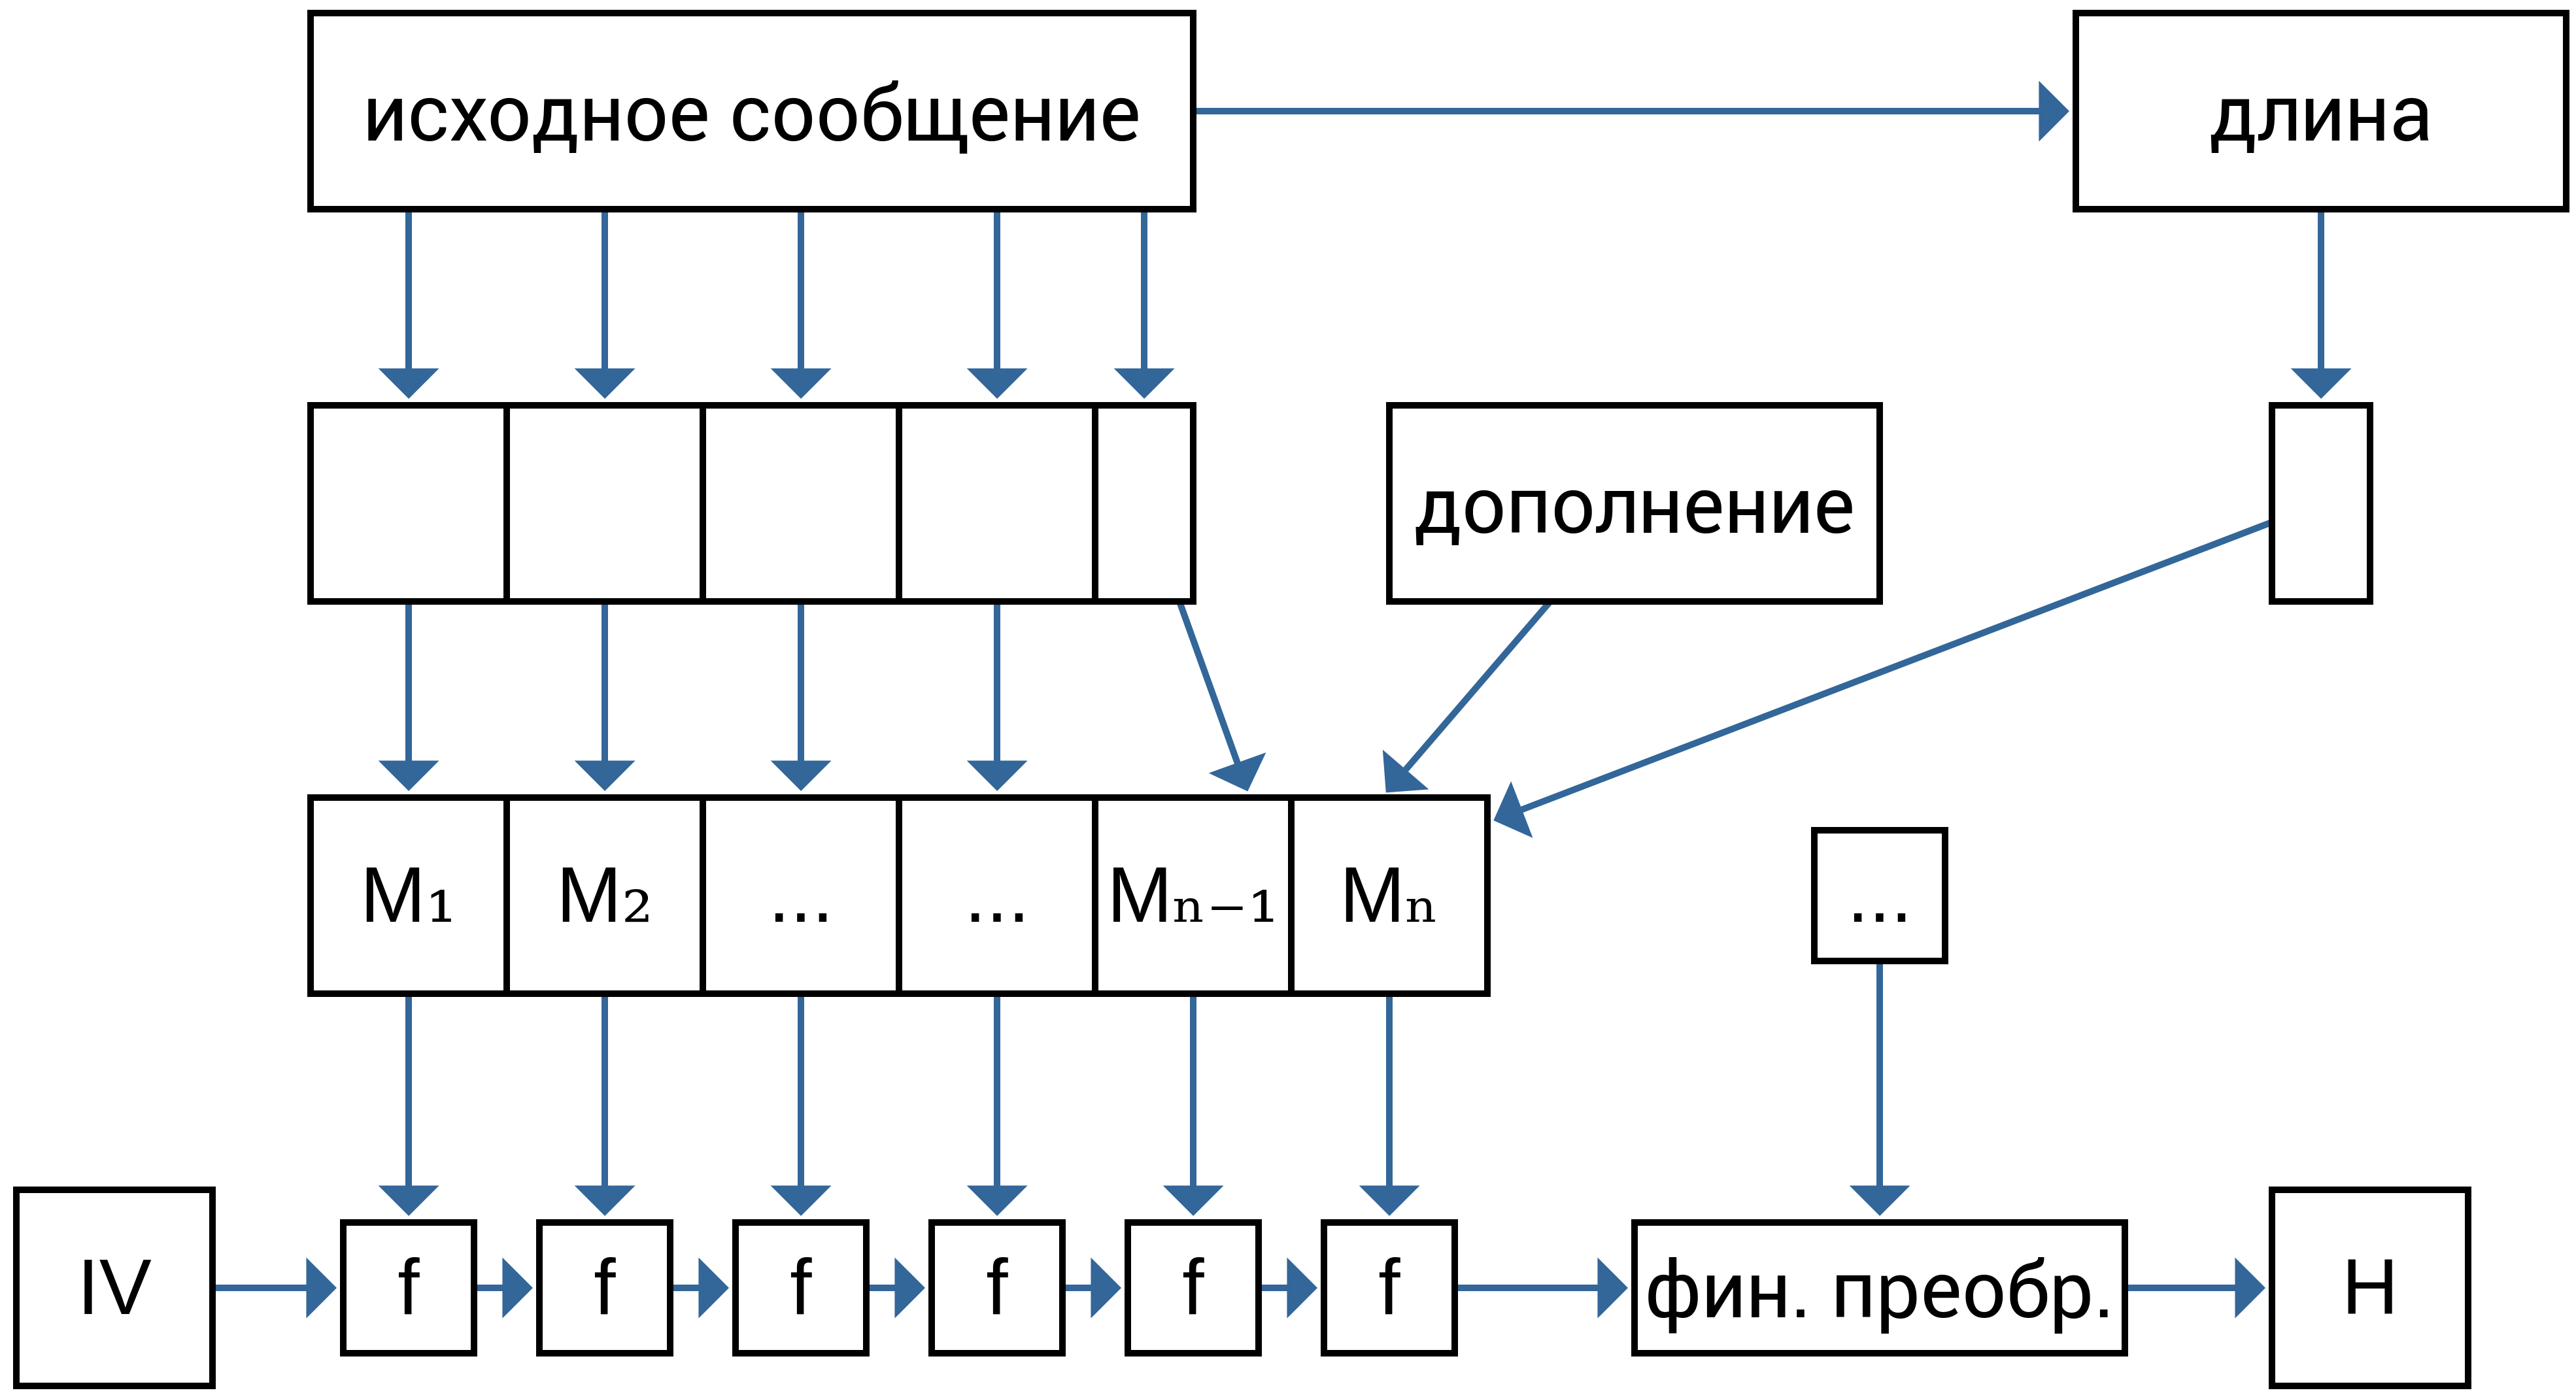
\includegraphics[width=0.95\textwidth]{pic/merkle-damgard}
    \caption{Структура Меркла~---~Дамгора}
    \label{fig:merkle-damgard}
\end{figure}

Пусть есть задан открытый текст $M$ в виде двоичной последовательности некоторой длины. Текст дополняется, во-первых, дополнением (паддингом), во-вторых, длиной исходного сообщения таким образом, чтобы после дополнения обрабатываемая последовательность можно было разбить на целое число блоков фиксированной длины $M_1, M_2, \dots, M_n$.

Выбирается некоторый начальный вектор IV. Далее последовательно применяется раундовая функция сжатия к двум аргументам, первым из которых является рещультат предыдущего вызова (IV для самого первого), а вторым аргументом -- соответствующий блок $M_i$ обрабатываемой последовательности.

\[\begin{array}{l}
H_0 = \text{IV},\\
H_i = f ( H_{i-1}, M_i ).\\
\end{array}\]

В зависимости от хеш-функции структура может быть дополнена финальным преобразованием, в котором вторым аргументом будет ещё одна некоторая функция от исходного сообщения. Например, в хеш-функции <<Стрибог>>\index{хеш-функция!Стрибог} таким аргументом является арифметическая функция всех блоков исходного открытого текста.

К плюсам данной конструкции относят доказанный авторами факт, что если раундовая функция сжатия устойчива к коллизиям, то итоговая хеш-функция будет также устойчива. Однако у конструкции присутствуют и недостатки.

\begin{itemize}
  \item Атака на нахождение второго прообраза (для некоторого известного открытого текста) может быть выполнена за $2^n / | M |$ операций, где $| M |$ -- длина открытого текста. Это меньше, чем требуется операций для полного перебора ($2^n$), особенно для длинных сообщений.
  \item Если известен способ нахождения пары коллизий, то множественные коллизии найти незначительно сложнее.
  \item В отсуствие финального преобразования при заданном значении хеш-функции $h = H(M)$ (и неизвестном исходном сообщении $M$) можно легко найти значение $H( pad(M) \| M' )$, где $pad(M)$ -- функция дополнения, а $M'$ -- выбранный злоумышленником дополнительный текст к исходному сообщению.
\end{itemize}

С использованием данной конструкции построены такие криптографические хеш-функции, как MD4\index{хеш-функция!MD4}, SHA-1\index{хеш-функция!SHA-1}, SHA-2\index{хеш-функция!SHA-2}, российский стандарт ГОСТ~Р~34.11-2012 (<<Стрибог>>)\index{хеш-функция!Стрибог} и многие другие.

\index{структура!Меркла~---~Дамгора|)}